% Building and training deformable models of objects (e.g. faces, ears, bodies, bottles, vehicles etc.) has recently been widely researched for object detection, part localisation, fitting, recognition and tracking using manual annotated data. Shapes and appearances of majority of objects vary significantly from object instance. To illustrate, ears have complicated inner structures (e.g. helix, crus antihelicis, scapha, tragus, lobe etc.) which differs remarkably between ears and highly sensitive to intensity changes. Recently, we have witnessed a great progress in object detection, alignment and recognition.

% To train deformable models with satisfiable generalisation, large amount of careful manual annotation is required. However, landmark annotation is extremely time consuming, work intensive and, most importantly, number of landmarks have to stay consistent for all training data while it is challenging to maintain the consistency or to avoid bias when annotating objects that having reach features. In ears, for example, large amount of landmarks required as the inner structure of ears are complex. To annotate an ear with clear contour, helix and cavum conchae, more than 50 landmarks are required. The inconsistency of ear features enhanced the difficulty of accurate annotation (e.g. Fossa Triangularies and Crus Helicis are optional feature of an ear also their visibility is highly sensitive to pose and illumination variation).
% To illustrate how much time consuming careful ear annotation is, according to our experience, a trained annotator may need an average of (TODO: experiment) minutes per image for the manual annotation of 55 landmarks. This means that the annotation of 1000 images requires a total of about (TODO: experiment). Furthermore, personal issue, prior knowledge and circumstances can heavily bias the annotation accuracy thus second round correction might desired.

% We propose a framework to (1) construct SDMs using training data with inconsistent annotation, (2) introduce highly effective curve annotation which tremendously reduces manual work overload but maintains same performance level against state-of-the-art SDMs and (3) build dense correspondent SDMs with shape flow.

% %(1)
% Annotated data of same objects can have various number of landmarks, \cite{?} shown faces have landmarks different in range 10+ to 70+. Building SDMs (e.g. Active Appearance Models), however, require training data are annotated consistently, for example, all faces have 68 landmarks, 6 landmarks for an eye and 9 for a nose \cite{?}. Such property of SDMs largely limited their application area like combining different dataset as one. We propose the pipeline with non-rigid alignment and support vector shape to blend landmarks into relatively consistent shape discriminator before building models.

% %(2)
% Due to the fact that manual annotation is a rather costly and labour-intensive procedure, unsupervised and semi supervised learning of models for the tasks of alignment, landmark localization, tracking and recognition has attracted considerable attention \cite{?}. As our proposed framework are available to handle landmarks with inconsistency, it leads to a more efficient, convenient, unbiased and simple annotation methods - curve annotation.

% %(3)
% To build dense correspondence between independent shapes, we apply optical flow on shapes with low rank constrains, so we name it shape flow. Optical flow is originally applied to video sequences that several assumptions holds, illumination consistency and motion smoothness, while shapes having no motion smoothness completely as all training data are independent. Low rank constrain plays important role to simulate motion smoothness assumption.


% % Back Ground, uses Nondas' paper "Automatic Construction of Deformable Models In-The-Wild" as place holder
% The two most closely related works to the proposed
% method are the automatic construction of Active Appearance
% Models (AAMs) in \cite{?} and the so-called RASL
% methodology in \cite{?} for person-specific face alignment.
% There are two main differences between our framework
% and \cite{?}. (1) We use a predefined statistical shape model
% instead of trying to find both the shape and appearance models.
% We believe that with the current available optimization
% techniques, it is extremely difficult to simultaneously optimize
% for both the texture and shape parameters. (2) We
% employ the robust component analysis of \cite{?} for the appearance
% which deals with outliers. Thus, even though
% our method is similar in concept to \cite{?}, these two differences
% make the problem feasible to solve. In particular, the
% methodology in \cite{?} fails to create a generic model even in
% controlled recording conditions, due to extremely high dimensionality
% of the parameters to be found and to the sensitivity
% of the subspace method to outliers. This was probably
% one of the reasons why the authors demonstrate very
% limited and only person-specific experiments. Furthermore,
% our methodology bypasses some of the limitations of \cite{?},
% which requires the presence of only one low-rank subspace,
% hence it has been shown to work only for the case of congealing
% images of a single person. Finally, we argue that
% in order for an automatically constructed AAM methodology
% to be robust to both within-class and out-of-class outliers4,
% which cannot be avoided in totally unsupervised setting
% statistical component analysis techniques should be
% employed \cite{?}.

% We summarize our contributions as follows:
% \begin{itemize}
%   \item Constructing SDMs using training data with inconsistent annotation.
%   \item Introduce highly effective curve annotation which tremendously reduces manual work overload but maintains same performance level against state-of-the-art SDMs.
%   \item Building dense correspondent SDMs with shape flow
% \end{itemize}

% In our experiment, we show that building robust dense models trained with inconsistent annotation and trained with curve annotation improves performance of discriminative models trained on carefully annotated data including ears, faces, bottles, (cars ?) and bodies. Evaluation methods and choices are described in details.


% \clearpage

\begin{figure}[t!]
    \centering
    \begin{subfigure}[b]{0.115\textheight}
            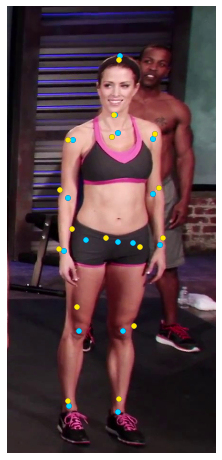
\includegraphics[height=2cm]{resources/MotivativeAnnotation/MPII}
    \end{subfigure}
    \hfill
    \begin{subfigure}[b]{0.115\textheight}
            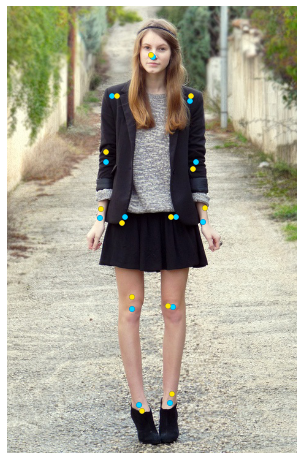
\includegraphics[height=2cm]{resources/MotivativeAnnotation/FashionPose}
    \end{subfigure}
  	\hfill
    \begin{subfigure}[b]{0.115\textheight}
            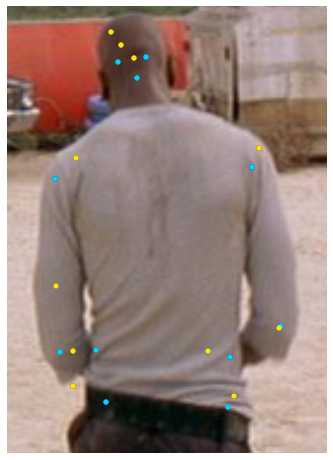
\includegraphics[height=2cm]{resources/MotivativeAnnotation/FLIC}
    \end{subfigure}
    \hfill
    \begin{subfigure}[b]{0.115\textheight}
            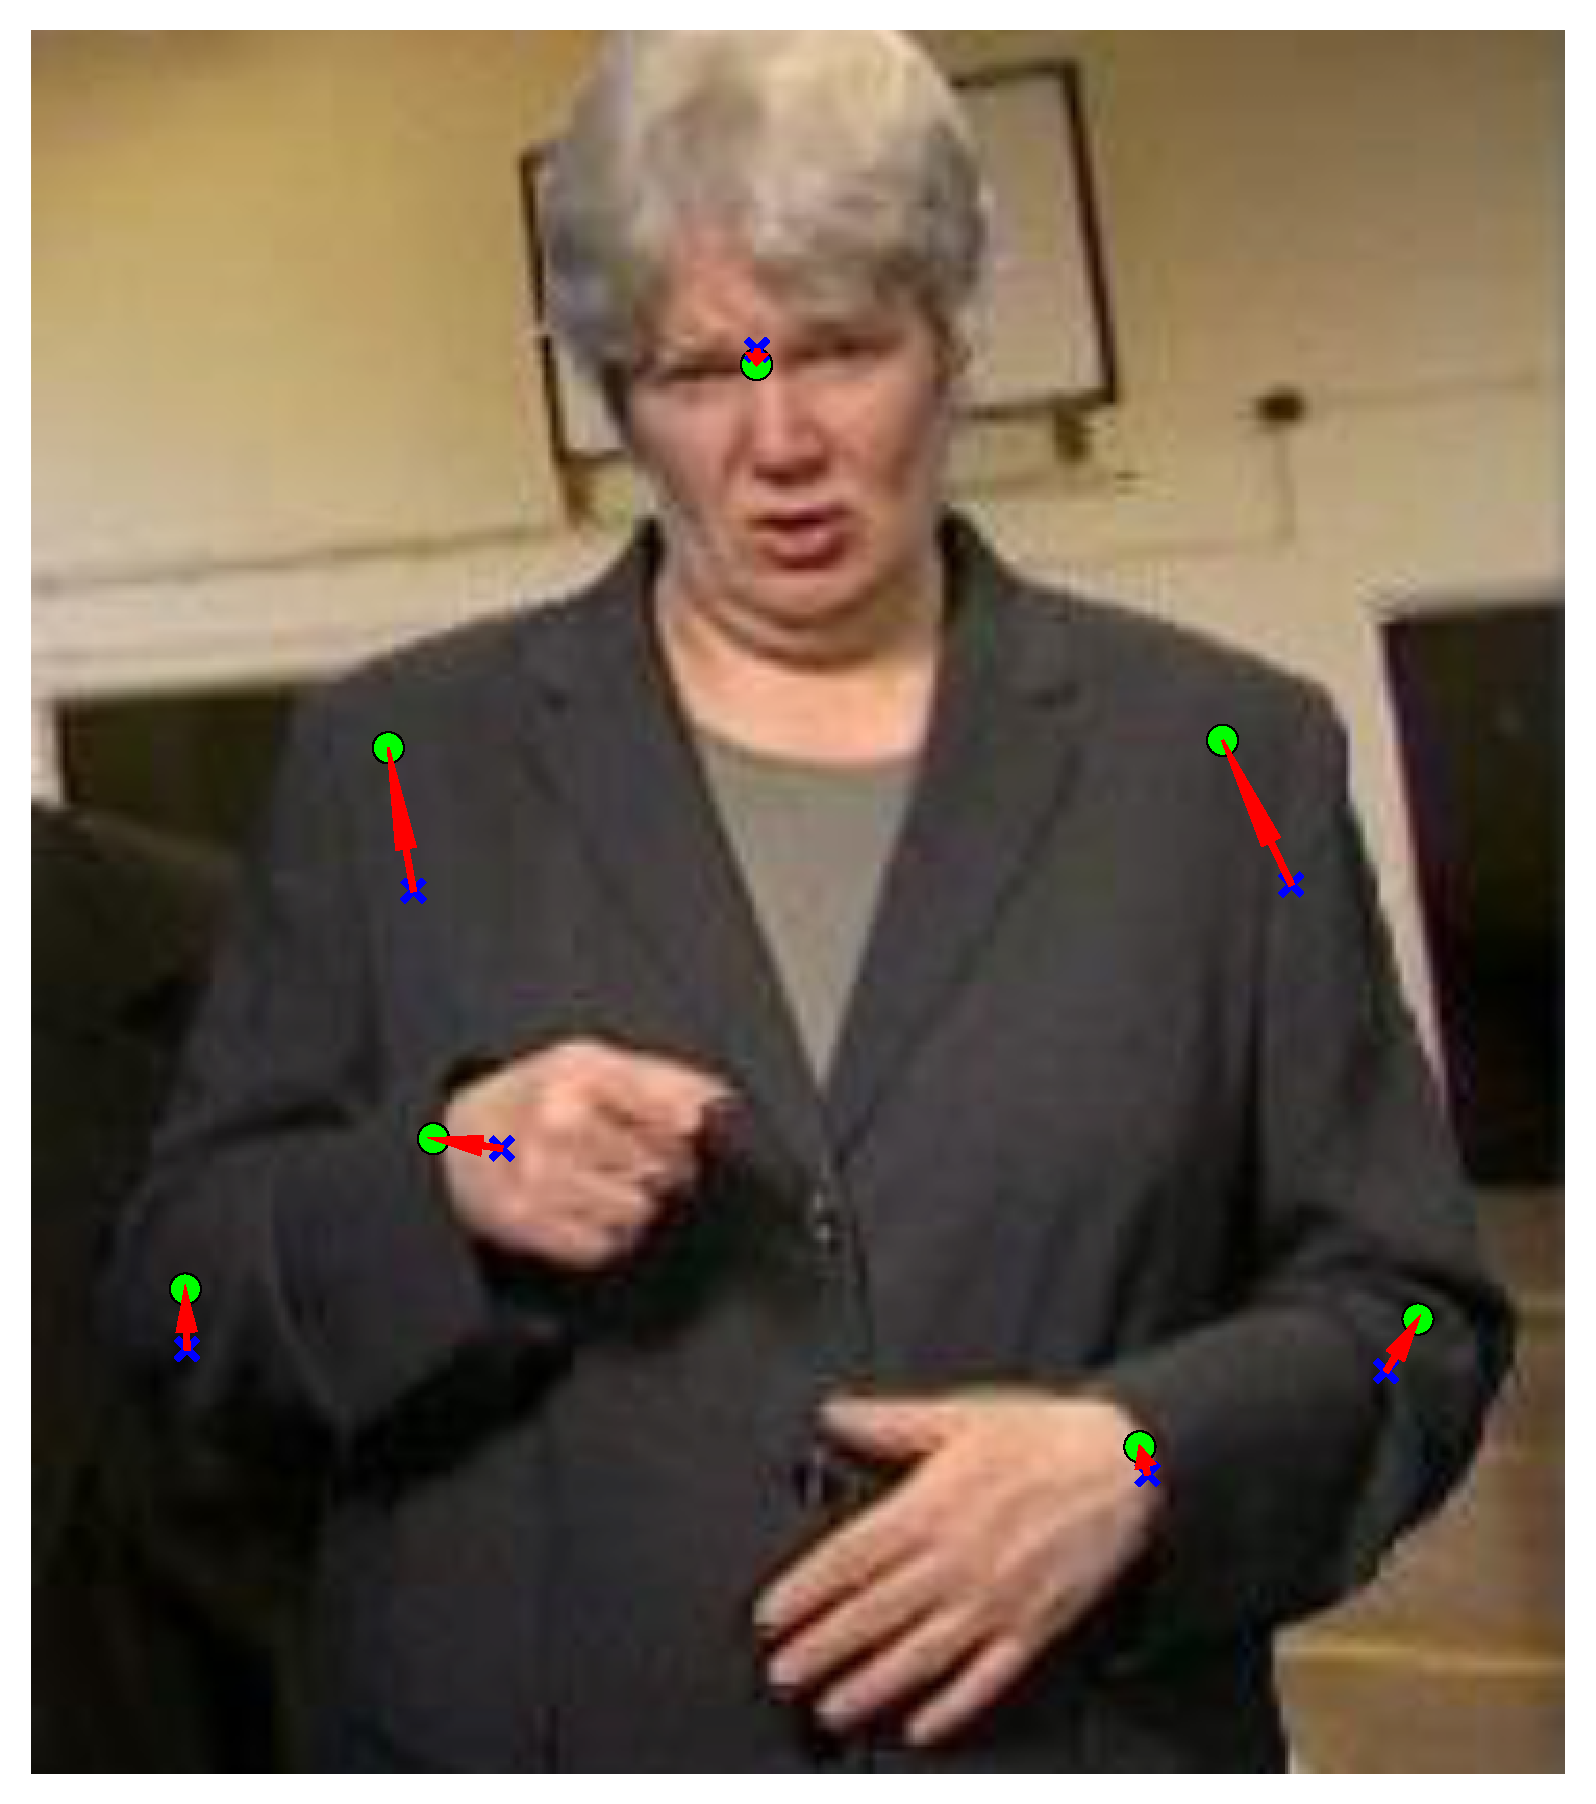
\includegraphics[height=2cm]{resources/MotivativeAnnotation/BBCPose}
    \end{subfigure}
    \\
    \begin{subfigure}[b]{0.08\textwidth}
            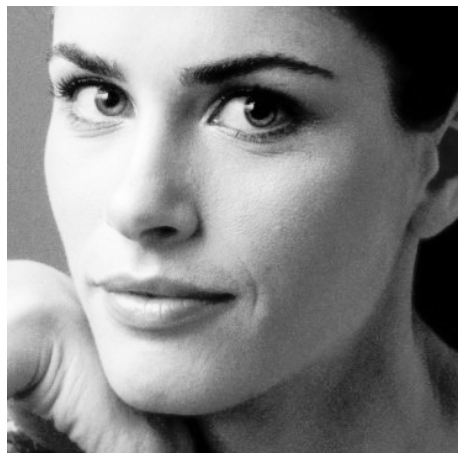
\includegraphics[width=\textwidth]{resources/Fig_Intro/intro_0_0}
    \end{subfigure}
    \hfill
    \begin{subfigure}[b]{0.08\textwidth}
            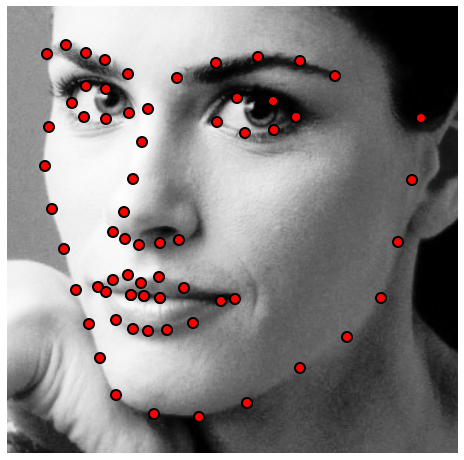
\includegraphics[width=\textwidth]{resources/Fig_Intro/intro_0_1}
    \end{subfigure}
  	\hfill
    \begin{subfigure}[b]{0.08\textwidth}
            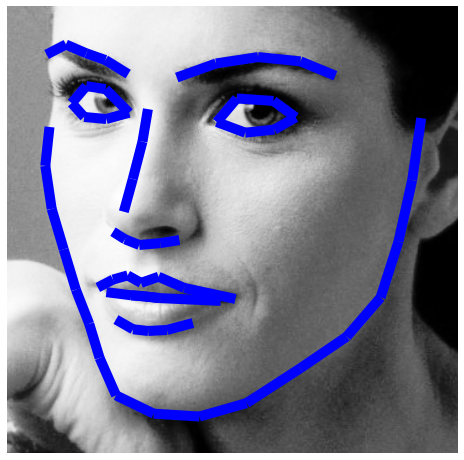
\includegraphics[width=\textwidth]{resources/Fig_Intro/intro_0_2}
    \end{subfigure}
    \hfill
    \begin{subfigure}[b]{0.08\textwidth}
            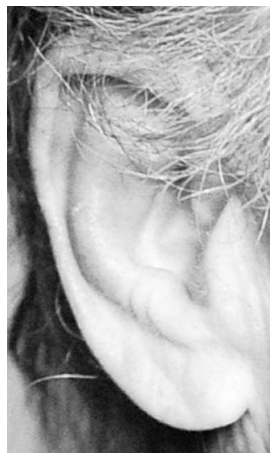
\includegraphics[width=\textwidth]{resources/Fig_Intro/intro_1_0}
    \end{subfigure}
    \hfill
    \begin{subfigure}[b]{0.08\textwidth}
            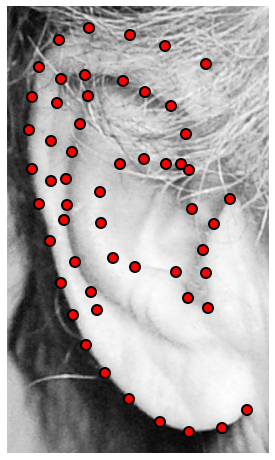
\includegraphics[width=\textwidth]{resources/Fig_Intro/intro_1_1}
    \end{subfigure}
    \hfill
    \begin{subfigure}[b]{0.08\textwidth}
            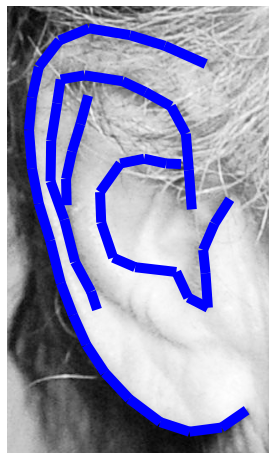
\includegraphics[width=\textwidth]{resources/Fig_Intro/intro_1_2}
    \end{subfigure}
    
    \caption{Demonstration of classical landmark annotation and curve annotation of faces, ears, bottles and human actions.}
    \label{fig:intro}
\end{figure}


Building and fitting statistical deformable models of objects is a well-studied and popular area in the intersection of computer vision and machine learning \cite{Cootes1995, Cootes2001, Matthews2004, Saragih2011, Belhumeur2011, Zhu2012, Xiong2013}. Recently, we have witnessed tremendous developments in building and fitting models of human faces and bodies using images captured in unconstrained recording environments, usually referred to as "in-the-wild" \cite{Belhumeur2011, Cao2012, Zhu2012, Xiong2013, Asthana2013, Tzimiropoulos2014, Asthana2014}. This is attributed to:
\begin{itemize}


\item The abundance of complex visual data, spread mostly through the Internet via web services such as Youtube, Flickr and Google Images. The latter has led to the development of large databases of "in-the-wild" images of human faces and bodies \cite{Belhumeur2011, Le2012, Zhu2012, Burgos2013}.

\item The development of powerful visual features, able to describe objects and its parts in a robust manner (e.g., Scale Invariant Feature Transforms (SIFT) \cite{lowe1999object}, Histogram of Oriented Gradients (HoGs) \cite{Dalal2005} and recently Deep Convolutional Neural Networks \cite{sermanet2013overfeat}), as well as generative and discriminative methodologies for learning deformable models.

\item Equally important is the task of manual annotation of images with regards to face and body parts and that has been undertaken by several research teams \cite{sagonas_iccv_300w_2013,charles2013domain,dantone2014body,andriluka14cvpr}.

\end{itemize}

There are two drawbacks on building deformable models that directly rely on landmarks:
\begin{itemize}

\item Annotating with regards to consistent landmark annotation is an extremely time consuming, tedious and labour intensive work \cite{sagonas_iccv_300w_2013}, which is usually performed by a trained person . Furthermore, for many objects it requires a highly skilled person to identify and annotate a set of images with regards to a consistent set of landmarks. For example human ears have very complicated inner structures (e.g. helix, crus antihelicis, scapha, tragus, lobe etc.) which differs remarkably between ears. Moreover, certain ear parts, such as  Fossa Triangularies and Crus Helicis, do not appear in all ears and  their visibility is highly sensitive to pose and illumination variation. Another example is human body which is generally annotated with regards to a number of landmarks that intuitively correspond to a set of body joints. The task of annotation was undertaken by a crowd-sourcing Internet marketplace, so-called Amazon Mechanical Turk (AMT). Unfortunately, these annotations are, in many cases, not consistent\footnote{From personal experience the quality of annotations that have been produced from AMT in case of faces are extremely inaccurate and cannot by any means compared with the ones provided by the recent competition \cite{sagonas_iccv_300w_2013}} (please see Figure \ref{fig:intro}). As it was also pointed out recently, the inconsistencies in body joint annotations may also render the comparison between different human pose estimation methodologies irrelevant \cite{tompson2015efficient}. 

\item The nature of many deformable objects does not allow them to be consistently annotated with regards to a consistent set of landmarks (e.g. bottles, fruits etc.). Also the boundary/outline of objects, such as faces, ears, body can be very difficultly annotated consistently. That is why many state-of-the-art methods opt to leave the boundary out for comparison \cite{Tzimiropoulos2014, Asthana2014}. The majority of the state-of-the-art methods for model-based landmark localisation \cite{Cao2012, Zhu2012, Xiong2013, Tzimiropoulos2014, Asthana2014} are not applicable for objects with inconsistent sets of landmarks.

\end{itemize}

To illustrate how time consuming careful annotation of the human ear is we lay down our own experience. A trained annotator needs an average of 4 minutes per image for the manual annotation of 55 landmarks. This means that the annotation of 1000 images requires a total of about 67 hours. Furthermore,  training and fatigue largely influence the annotation accuracy. Hence, a second pass on the annotated data is, in many cases, necessary. Due to the fact that manual annotation is a costly and labour-intensive procedure, unsupervised learning of deformable models for the tasks of object alignment has recently attracted some attention \cite{frey2003learning, baker2004automatic, cootes2004groupwise, jojic2006escaping, Huang2006, kokkinos2007unsupervised, jiang2009learning, liu2009simultaneous, Zhang2012}. However, because the problem of fully unsupervised discovery of the deformations of arbitrary objects is difficult and ill-posed the limited number of methods that have been applied to the task cannot be directly applied to arbitrary collection of images collected "in-the-wild". On the other hand, the method of \cite{antonakos2014automatic}, which can deal with "in-the-wild" images, requires a set of consistently annotated sparse shapes to perform deformable face congealing.


In this paper, we provide a solution for annotating an object with regards to its deformations that requires considerable less effort and in the same time can be used to define statistical deformations for objects without consistent set of landmarks. We apply the proposed method to construct deformable models of the outline of  human body parts (e.g., arms and legs). To the best of our knowledge this is the first SDM of the outline of human body parts. The proposed SDM can be also used to provide accurate and consistent annotations of several of the body joints (such as wrist etc.). 

To this end, we argue and empirically demonstrate that it is better to annotate an object with regards to a set of continuous lines that describe the shape of the object. An example is provided in Figure \ref{fig:intro} where the shape of the human arm is annotated with continuous lines instead of a number of discrete landmarks. Similarly, the shape annotations for the ear, a bottle and human body is shown in Figure \ref{fig:intro} Annotating facial images by following this procedure takes 42, 38 and 43 secs per image for arm, faces, ears and bottles correspondingly. Furthermore, these shapes can be automatically produced by recent methods that perform discriminative segmentation of objects.

Furthermore, we show that flow methods have mature enough so that it can be used to densely annotate the proposed shapes using simple, as well as more recent and robust shape representations methods \cite{Garg:2013hu,Nguyen2013}.  In particular, to build dense correspondence between independent shapes, we apply optical flow on shapes with low rank constrains, so we name it shape flow. Optical flow is originally applied to video sequences that several assumptions holds, illumination consistency and motion smoothness, while shapes having no motion smoothness completely as all training data are independent. Low rank constrain plays important role to simulate motion smoothness assumption.

We show that this way dense correspondences between images can be established and dense Active Appearance Models (AAMs) can be build on top of that. We show that the proposed methodology even though not tailored to landmark localization can be applied for landmark localization achieving very good performance. We demonstrate the performance of the proposed methodology for describing objects that do not have consistent landmarks. Furthermore, We show that by sampling the shape of the dense AAM a part-based AAM can be trained with its parts being in correspondence. We show that such a part-based AAM can used to produce state-of-the-art results in localisation of human body parts in challenging database, outperforming state-of-the-art methods [..]. Finally, we show that the proposed part-based AAM can be used to provide consistent annotations for certain body parts. 


%To the best of our knowledge this is the first methodology which can %create a dense statistical model for AAM which can operate in %"in-the-wild".

%[..]. There are methods such as [..] and [..] but ...


Summarizing, the contributions proposed in this paper are:
\begin{itemize}

  \item We propose one of the first methodologies that construct SDMs from a set of training data with inconsistent annotation. We show that the proposed methodology, since it uses highly effective curve annotation, tremendously reduces manual work overload but maintains same performance level against state-of-the-art SDMs. We show that by sampling the dense shape of SDM very powerful part-based SDMs can   
  
  \item We propose the first SDMs of the outline of human parts, such as human arms, which can be applied for both highly accurate body part segmentation and pose estimation, as well as for providing accurate annotations for body joints. 
  
\end{itemize}



%In our experiment, we show that building robust dense models trained with inconsistent annotation and %trained with curve annotation improves performance of discriminative models trained on carefully %annotated data including ears, faces, bottles, (cars ?) and bodies. Evaluation methods and choices are %described in details.




%We propose a framework to (1) construct SDMs using training data with inconsistent annotation, (2) %introduce highly effective curve annotation which tremendously reduces manual work overload but %maintains same performance level against state-of-the-art SDMs and (3) build dense correspondent SDMs %with shape flow.

%(1)
%Annotated data of same objects can have various number of landmarks, \cite{?} shown faces have %landmarks different in range 10+ to 70+. Building SDMs (e.g. Active Appearance Models), however, %%require training data are annotated consistently, for example, all faces have 68 landmarks, 6 landmarks %for an eye and 9 for a nose \cite{?}. Such property of SDMs largely limited their application area like %combining different dataset as one. We propose the pipeline with non-rigid alignment and support vector %shape to blend landmarks into relatively consistent shape discriminator before building models.

%(2)



%(3)


% Back Ground, uses Nondas' paper "Automatic Construction of Deformable Models In-The-Wild" as place holder
%The two most closely related works to the proposed
%method are the automatic construction of Active Appearance
%Models (AAMs) in \cite{?} and the so-called RASL
%methodology in \cite{?} for person-specific face alignment.
%There are two main differences between our framework
%and \cite{?}. (1) We use a predefined statistical shape model
%instead of trying to find both the shape and appearance models.
%We believe that with the current available optimization
%techniques, it is extremely difficult to simultaneously optimize
%for both the texture and shape parameters. (2) We
%employ the robust component analysis of \cite{?} for the appearance
%which deals with outliers. Thus, even though
%our method is similar in concept to \cite{?}, these two differences
%make the problem feasible to solve. In particular, the
%methodology in \cite{?} fails to create a generic model even in
%controlled recording conditions, due to extremely high dimensionality
%of the parameters to be found and to the sensitivity
%of the subspace method to outliers. This was probably
%one of the reasons why the authors demonstrate very
%limited and only person-specific experiments. Furthermore,
%our methodology bypasses some of the limitations of \cite{?},
%which requires the presence of only one low-rank subspace,
%hence it has been shown to work only for the case of congealing
%images of a single person. Finally, we argue that
%in order for an automatically constructed AAM methodology
%to be robust to both within-class and out-of-class outliers4,
%which cannot be avoided in totally unsupervised setting
%statistical component analysis techniques should be
%employed \cite{?}.

